\section{Conic Sections}
  Parabolas, ellipses, and hyperbolas are called \textbf{conic sections}, or \textbf{conics}, because they result from intersecting a cone with a plane.
  \begin{center}
    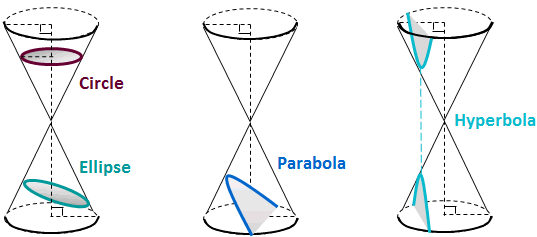
\includegraphics[width=300pt]{conics.png}
  \end{center}
  \subsection*{Parabolas}
    A \textbf{parabola} is the set of points in a plane that are equidistant from a fixed point $F$ (called the \textbf{focus}) and a fixed line (called the \textbf{directrix}). The halfway point between the focus and directrix is on the parabola and is called the \textbf{vertex}. The line through the focus and the vertex and perpendicular to the directrix is the \textbf{axis} of the parabola.
    \begin{center}
      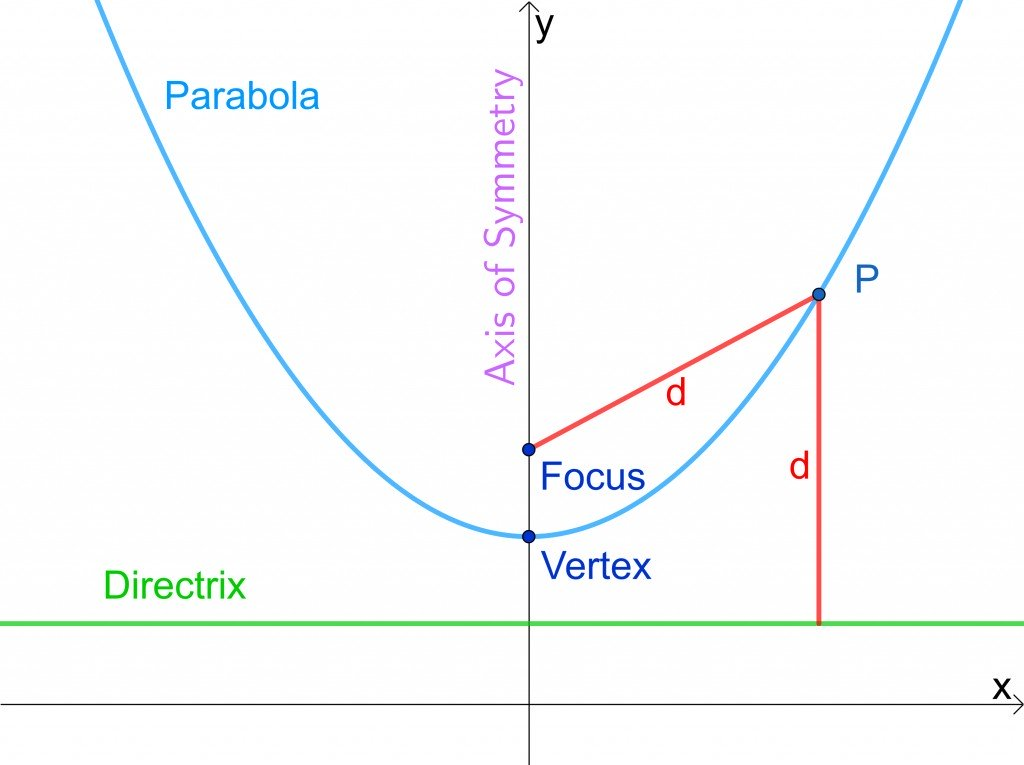
\includegraphics[width=200pt]{parabola.jpg}
    \end{center}
    As seen in the figure, the focus is always inside the region of the parabola and the directrix is the same distance away on the opposite side.
    \begin{definition}
      An equation of the parabola with focus $(0,p)$ and directrix $y=-p$ is $$x^2=4py$$. If we set $a=\frac{1}{4p}$, then the standard equation of a parabola is $y=ax^2$. This opens upward if $p>0$ and downard if $p<0$, and is symmetric with respect to the y-axis.
    \end{definition}
    \begin{definition}
      If we switch $x$ and $y$, we get $$y^2=4px$$ (reflection about the diagonal line y=x). This parabola opens to the right if $p>0$ and to the left if $p<0$.
    \end{definition}
    \begin{definition}
      The vertex form of a parabola is
      $$y=a(x - h)^2 + k$$
      where $(h, k)$ is the vertex of the parabola and $x=h$ is the axis of symmetry. We can also switch $x$ and $y$ to get the vertex form of the rotated parabola.
    \end{definition}
    \begin{example}
      Find the focus and directrix of the parabola $y^2 + 10x = 0$.
    \end{example}
    \begin{solution}
      We rewrite the equation as $y^2=-10x$. We know $y^2=4px$, so $4px=-10x$ and $p=-\frac{5}{2}$. Thus, the focus is $(p,0)=-\frac{5}{2},0)$ and the directrix is $x=\frac{5}{2}$.
    \end{solution}
  \subsection*{Ellipses}
    An \textbf{ellipse} is the set of points in a plane surrounding two fixed focal points $F_1$ and $F_2$ such that the \underline{sum} of the two distances to the focal points is a constant. Imagine tracing a line along the furthest path of a string stretched across two different points.
    \begin{definition}
      The ellipse $$\frac{x^2}{a^2}+\frac{y^2}{b^2}=1 \ \ \ a \geq b \geq 0$$ has foci $(\pm c,0)$, where $c^2=a^2 - b^2$, and vertices $(\pm a,0)$ \textbf{(lies on x-axis)}.
    \end{definition}
    The \textbf{vertices} are on the \textbf{major axis}, where $a$ is the distance to the center of the ellipse from each vertex. This distance is greater than the distance from a \textbf{co-vertex} to the center of the ellipse, $b$. The co-vertices lie on the \textbf{minor axis}. Because the sum of the two distances from a point on the ellipse to the foci is a constant, the distance from a co-vertex to a focal point is also $a$. If the foci coincide, then $c=0$, so $a=b$ and the ellipse becomes a circle with radius $r=a=b$.
    \begin{definition}
      The ellipse $$\frac{x^2}{b^2}+\frac{y^2}{a^2}=1 \ \ \ a \geq b \geq 0$$ has foci $(0, \pm c)$, where $c^2=a^2 - b^2$, and vertices $(0, \pm a)$ \textbf{(lies on y-axis)}.
    \end{definition}
    \begin{definition}
      The general form of a horizontal ellipse is
      $$\frac{(x-h)^2}{b^2}+\frac{(y-h)^2}{a^2}=1$$
      where $(h,k)$ is the center of the ellipse. The same transformation can be done to the standard form of a vertical ellipse.
    \end{definition}
    \begin{center}
      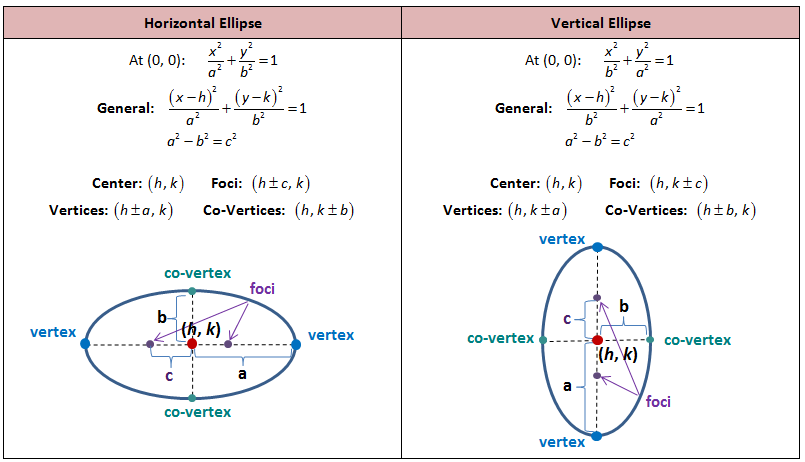
\includegraphics[width=300pt]{ellipse.png}
    \end{center}
    \begin{example}
      Find an equation of the ellipse with foci $(0,\pm 2)$ and vertices $(0, \pm 3)$.
    \end{example}
    \begin{solution}
      This equation represents a vertical ellipse because the foci and vertices lie on the $y$-axis. The distance from a focal point to the center is $c=2$ and the distance from a vertex to the center is $a=3$. Then we obtain $b^2=a^2 + c^2=9-4=5$, so the equation of the ellipse is
      $$\frac{x^2}{b^2}+\frac{y^2}{a^2}=\frac{x^2}{5}+\frac{y^2}{9}=1$$
    \end{solution}
  \subsection*{Hyperbolas}
    An \textbf{ellipse} is the set of points in a plane surrounding two fixed focal points $F_1$ and $F_2$ such that the \underline{difference} of the two distances to the focal points is a constant. The \textbf{transverse axis} is the axis of a hyperbola that passes through the two foci. The \textbf{conjugate axis} is perpendicular to the transverse axis and passes through the center of the hyperbola.
    \begin{center}
      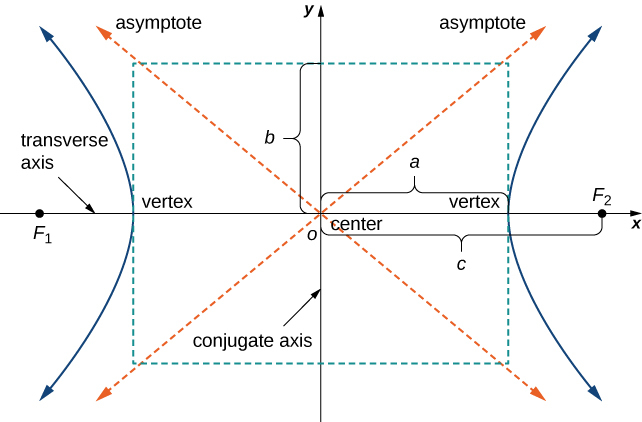
\includegraphics[width=200pt]{hyperbola.jpg}
    \end{center}
    \begin{definition}
      The hyperbola along a horizontal transverse axis
      $$\frac{x^2}{a^2}-\frac{y^2}{b^2}=1$$
      has foci $(\pm c,0)$, where $c^2=a^2 + b^2$, vertices $(\pm a,0)$ \textbf{(lies on x-axis)}, and asympotes $y=\pm\frac{b}{a}x$.
    \end{definition}
    \begin{definition}
      The hyperbola along a vertical transverse axis
      $$\frac{y^2}{a^2}-\frac{x^2}{b^2}=1$$
      has foci $(0, \pm c)$, where $c^2=a^2 + b^2$, vertices $(0, \pm a)$ \textbf{(lies on y-axis)}, and asympotes $y=\pm\frac{a}{b}x$.
    \end{definition}
     \begin{definition}
      The general form of a hyperbola along a horizontal transverse axis is
      $$\frac{(x-h)^2}{b^2}-\frac{(y-h)^2}{a^2}=1$$
      where $(h,k)$ is the center of the ellipse. The same transformation can be done to the standard form a hyperbola along a vertical transverse axis.
    \end{definition}
    \begin{example}
      Find the foci and asymptotes of the hyperbola ${9x^2 - 16y^2 = 144}$.
    \end{example}
    \begin{solution}
      If we divide both sides of the equation by 144, it becomes $$\frac{x^2}{16}-\frac{y^2}{9}=1$$
      which is a hyperbola along a horizontal transverse axis. Therefore, we get $a=4$ and $b=3$. Since $c^2=a^2 + b^2 = 16+9=25$, $c=5$. The foci are $(\pm 5,0)$, and the asymptotes are $y=\pm\frac{3}{4}x$.
    \end{solution}